% Drawing 148/02-2 -- folder 148, batch 02, archive page 22 (PDF page 23).
% Transcription: en haut à gauche, un tétraèdre à l'encre, les quatre sommets marqués de gros points, l'arête cachée en tirets ; une flèche de rotation épaisse autour du sommet de droite, un arc au crayon autour du sommet du haut, de petites marques (flèches) sur les arêtes issues du sommet du haut.
% Kind: tetrahedron with a rotation arrow at one vertex. Method 2 (schematic redraw from the facsimile). Status: partial.
% Notes: Four vertices as heavy dots (the top one the largest), five edges solid and the hidden edge (lower left to right) dashed, all between the same four points; the edge from the top to the lower right vertex is bowed on the page and drawn straight. A heavy curved arrow turns around the right vertex; a pencil arc passes over the top vertex. Small marks on the three edges from the top vertex, drawn as short arrows pointing away from it. Still differs: the direction of the small marks is a reading (two are blots, one is a small star), and the faint pencil ovals around the figure are left out. The note of the transcription puts the rotation arrow around the marked (top) vertex; on the page the heavy arrow is at the right vertex and only a pencil arc is at the top one. Redrawn 2026-11-12 (issue 128): to check again.
% Coordinates: 1 unit = 1 mm = 1/100 of the crop width, y downwards as on the crop (bbox in page fractions: [0.24, 0.29, 0.5, 0.42]).
% Redrawn by Claude (claude-fable-5-2), issue #128, 2026-11-12; not checked by a human; not compiled (no TeX in the session).
% Rights: reproduces part of the work -- behind RENDER_TRANSCRIPTS, never published by itself.
\documentclass[tikz,border=3pt]{standalone}
\usepackage{amsmath,amssymb}
\usetikzlibrary{patterns,arrows.meta}
\tikzset{pencil/.style={black!45}, struck/.style={black!35}, mpt/.style={circle,draw,inner sep=1.3pt}, pt/.style={circle,fill,inner sep=0.9pt}, opt/.style={circle,draw,fill=white,inner sep=1.1pt}, Rd/.style={red!75!black}, Gn/.style={green!45!black}, Br/.style={brown!70!black}}
\begin{document}
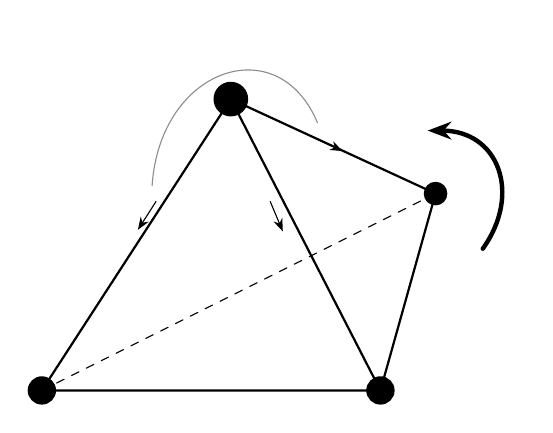
\begin{tikzpicture}[x=1mm,y=-1mm,line cap=round,line join=round,font=\small]
\coordinate (T) at (42,18);
\coordinate (R) at (68,30);
\coordinate (L) at (18,55);
\coordinate (B) at (61,55);
\draw[thick] (T) -- (R) -- (B) -- (L) -- cycle;
\draw[thick] (T) -- (B);
\draw[dashed] (L) -- (R);
\fill (T) circle [radius=2.2];
\fill (R) circle [radius=1.5];
\fill (L) circle [radius=1.8];
\fill (B) circle [radius=1.8];
\draw[line width=1.6pt,-{Stealth[length=3mm]}] (74,37) .. controls (79,30) and (76,22) .. (67,22);
\draw[pencil] (32,29) .. controls (33,14) and (48,9) .. (53,21);
\draw[-{Stealth[length=1.6mm]}] (52.4,22.8) -- (56.2,24.6);
\draw[-{Stealth[length=1.6mm]}] (32.5,31) -- (30.2,34.6);
\draw[-{Stealth[length=1.6mm]}] (47,31) -- (48.6,34.8);
\end{tikzpicture}
\end{document}
